
\par
Pierwsze tomografy komputerowe przeżyły swój rozkwit w latach siedemdziesiątych ubiegłego wieku.
Spowodowało to, że obrazu medyczne nie były bezpośrednim wynikiem badania, a jedynie wynikiem obróbki danych pomiarowych przez komputer.
Zwyczajne pliki graficzne (jak np. jpg, png, gif), nie nadawały się do zapisu takich obrazów, ponieważ zapisywały obraz w spektrum światła widzialnego w postaci składowych RGB.
Każdy producent stosował  własny format plików, który nie był upubliczniany.

\subsection{Standard DICOM v3.0}
\subsection{Standard DICOM v3.0}

\par
Standard DICOM jest odpowiedzią społeczności radiologów, radiofarmaceutów, fizyków medycznych na potrzebę wymiany danych pomiędzy różnymi systemami komputerowymi, przeglądarek obrazów,  stacji do przetwarzania i analizowania obrazów medycznych.

\par
Standard DICOM wersji trzeciej to standard definiujący ujednolicony sposób zapisu i przekazywania danych medycznych reprezentujących lub związanych z obrazami diagnostycznymi w medycynie.
Standard został wydany w 1993 przez dwie agencje ACR (American College of Radiology) i NEMA (National Electrical Manufactures Association).
Wcześniejsze wersje nazywały się ACR/NEMA v1.0, wydana w 1983 roku i ACR/NEMA v2.0, wydana w 1990 roku, stąd wersja trzecia.
Od wydania wersji trzeciej w 1993, standard jest wciąż rozwijany i uzupełniany o nowe elementy.
W obecnej chwili standard DICOM definiuje 81 różnych typów badań.

UWAGA: Za każdym razem kiedy jest odniesienie do obecnego standardu DICOM, w domyśle jest to odsłona 2019a.

\subsection{Sposób zapisu danych w pliku DICOM}

\par
Plik w formacie DICOM przypomina zbiór \enquote{elementów danych} z rekordami.
Zbiór nazywa się \keyword{Data Set} i składa się z rekordów, które nazywają się \keyword{Data Element}.
Elementy danych są ułożone w postaci listy.
Element danych może zawierać w sobie listę elementów danych.

\begin{figure}[!htbp]
    \centering
    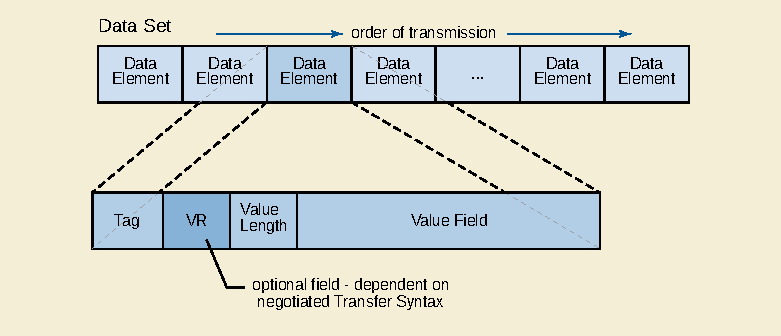
\includegraphics[]{img/dicom-dataelement001.pdf}
    \caption{Elementy danych w zbiorze elementów danych}
    \label{fig:dicom-dataelement}
\end{figure}

\subsubsection{Data Element}

\keyword{Data Element} jest rekordem, który przechowuje jakaś jedną informacje o czymś.
Składa się z czterem elementów:

\begin{itemize}

    \item \keyword{Tag} - to unikalny identyfikator, dalej zwany zanczniekiem, złożony z dwóch liczb: numer grupy (\cppcode{uint16}) i numer elementu (\cppcode{uint16}) grupy.
          Informuje o tym co dany rekord w sobie zawiera.
          W jednym zbiorze elementów nie mogą się pojawić dwa elementy posiadających ten sam znacznik.

          Na przykład: jeżeli liczby \keyword{Tag} przyjmą wartości odpowiednio wartość $0010_{16}$ i $0010_{16}$ to oznacza, że jest to tag \dicomtag{PatientName}{0010}{0010}, czyli zwiera w sobie parametr zawierają nazwę pacjenta.

          Dokładne omówienie \keyword{Tag}-ów znajduje się w dalszej części sekcji.

    \item \keyword{Value Representation}, w skrócie \keyword{VR} – to dwa bajty w postaci tekstu, informujący o formacie w jaki parametr został zapisany.

          Dokładne omówienie \keyword{VR}-ów znajduje się w dalszej części sekcji.

    \item \keyword{Value Length}, w skrócie \keyword{VL} - 32-bitowa lub 16-bitowa liczba nieoznaczona, która informuje o długości pola danych (\keyword{Value Field}).

          Wartość \keyword{VL} zwykle jest liczbą parzystą.
          Standard DICOM zakłada, że wszystkie dane powinny być dopełniane do parzystej liczby bajtów.

    \item \keyword{Value Field} (opcjonalne) - pole z parametrem o długości VL.

\end{itemize}

\subsubsection{Znacznik}
\label{sec:dicom-tag}

Tagi to unikalne znaczniki pozwalające określać co jest zapisane w \keyword{Data Element}.
Tag jest zrobiony z dwóch liczb: numeru grupy i numeru elementu.
Obie liczby to 16-bitowe liczby całkowite zapisywane w postaci  heksadecymalnej.

Istnieją dwa rodzaje znaczników: publiczne o parzystym numerze grupy i prywatne o nieparzystym numerze.
Pierwsza grupa jest definiowana przez standard DICOM, zawiera ona podstawowe znaczniki
Publiczne znaczniki dzielę się na obowiązkowe, opcjonalne i warunkowe.
Są określane przy definicji obiektów informacyjnych.
Natomiast druga grupa to tagi, pozostawione do dyspozycji producentom sprzętu, tak by mogli zapisywać dodatkowe informacje, które nie zostały przewidziane w standardzie DICOM.
Taki umożliwia podział umożliwia zapisywane ogromnej liczby informacji ustandaryzowanej jak i informacji niestandardowej w sposób bezkonfliktowy i z możliwosćią odczytania danych przez aplikacje nie związane z producentem sprzętu.

Obecna odsłona DICOM definiuje znaczenie ponad 4000 publicznych tagów z informacjami oraz jakie VR powinny mieć.
Oto kilka przykładów:
\begin{itemize}
    \item \dicomtag{PatientName}{0010}{0010} - nazwa pacjenta, tag który zawsze musi się pojawić, może być pusty w przypadku kiedy pacjent jest bezimienny

    \item \dicomtag{PatientID}{0010}{0020} - id pacjenta, unikalny identyfikator pacjenta, najczęściej jest to numer HIS(Hospital Information System)

    \item \dicomtag{PatientBirthDate}{0010}{0030} - data urodzenia pacjenta

    \item \dicomtag{PatientSex}{0010}{0040} - płeć pacjenta

    \item \dicomtag{PatientAge}{0010}{1010} - wiek pacjenta w czasie badania

    \item \dicomtag{StudyDescription}{0008}{1030} - opis badania, pole wypełniane przez technika lub lekarza

    \item \dicomtag{SeriesDescription}{0008}{103E} - ops serii, pole wypełniane przez technika lub lekarza

    \item \dicomtag{SeriesInstanceUID}{0020}{000E} - unikalny numer serii, jest nadawany każdemu badaniu

    \item \dicomtag{InstanceNumber}{0020}{0013} - numer instancji ramki, używany w przypadku kiedy z jednego badania zostało utworzonych kilka plików DICOM

    \item \dicomtag{Modality}{0008}{0060} - modalność określająca rodzaj techniki diagnostycznej

    \item \dicomtag{StudyDate}{0008}{0020} - data wykonania badania
\end{itemize}


\subsubsection{VR - Value Representation}
\label{sec:dicom-vr}

VR informuje w jakim formacie jest zapisany parametr obrazu.
Składa się z dwóch bajtów.

Przykładowe VR:
\begin{itemize}
    \item AS - Age String - wiek lub długość życia

          Długość danych zawsze wynosi 4 bajty.
          Pierwsze trzy bajty to liczba całkowita zapisana za pomocą tekstu.
          Czwarty bajt to znaku określający jednostkę czasu.
          Standard definiuje cztery możliwe jednostki czasu: \dataword{D} jako dzień, \dataword{W} jako tydzień, \dataword{M} jako miesiąc, oraz \dataword{Y} jako jeden rok.

          Przykład: \dataword{018M} oznacza 18 miesięcy, \dataword{123D} oznacza 123 dni.

    \item AT - Attribute Tag - inny tag

          Długość danych to zawsze 32 bity, są to dwie 16 bitowe liczby.
          Odpowiednio grupa i element grupy.
          Ten VR jest używany kiedy wskazujemy na inny tag.
          Wartość nie jest nigdy pokazywana użytkownikowi, a jedynie używana w interpretacji przez inne algorytmu do analizy obrazu.

          Przykład: tag \dicomtag{FrameIncrementPointer}{0028}{0009} jest używany kiedy w pliku jest zapisana sekwencja kilku obrazów, wskazuje on na inny tag zawierający informacje, w jaki sposób ta sekwencja ma być wyświetlona.

    \item DA - Date - data lub dzień

          Długość danych zawsze wynosi 8 bajtów.
          Data zapisana w formacie \dataword{YYYYMMDD}, gdzie: \dataword{YYYY} cztery cyfry roku, \dataword{MM} dwie cyfry miesiąca, \dataword{DD} dwie cyfry dnia w kalendarzu Gregoriańskim.

          Przykład: \dataword{19800716} oznacza 16 lipca 1980

          UWAGA: Standard \enquote{ACR-NEMA Standard 300}, czyli poprzednik DICOM definiował date w sposób \dataword{YYYY.MM.DD}, według standardu DICOM, taki zapis jest nie poprawny, ale zdarzają się stare obrazy z takimi datami i \sokarclass{DataConverter} obsługuje taki format.

    \item DS - Decimal String - liczba zmiennoprzecinkowa lub ciąg kilku liczb zmienno przecinkowych zapisanych za pomocą tekstu w notacji wykładniczej

          Długość jednej liczby powinna maksymalne wynosić 16 bajtów.
          Dostępne znaki to \dataword{0}-\dataword{9}, \dataword{+}, \dataword{-}, \dataword{E}, \dataword{e}, \dataword{.}.
          Biblioteka QT posiada wbudowany konwerter liczb zapisanych w formacie wykładniczym, dlatego mój konwerter dzieli tekst i konwertuje za pomocą QT.

          Przykład: \dataword{426\textbackslash468 } oznacza dwie liczby 426 i 468. Proszę zwrócić uwagę na spacje na końcu.

    \item IS - Integer String - liczba całkowita

          Długość jednej liczby powinna maksymalne wynosić 12 bajtów.
          Dostępne znaki to \dataword{0}-\dataword{9}, \dataword{+}, \dataword{-}.
          Biblioteka QT posiada wbudowany konwerter liczb całkowitych, dlatego mój konwerter używa konwertera z QT.

          Przykład: \dataword{426 }  oznacza liczbę 426.

    \item PN - Person Name - nazwa osoby

          Jako, że pacjenta, bądź obiekt badany można nazwać w sposób dowolny i odbiegający od polskiego standardu nazewnictwa, standard DICOM nie przewiduje rozdzielenia poszczególnych składowych nazwy na oznaczone fragmenty.
          \enquote{Person Name} dzieli nazwę na podane fragmenty, rozdzielony znakiem \dataword{\^{}} (94 znak kodu ASCII):
          \begin{itemize}
              \item family name complex - nazwisko, np. Smolik
              \item given name complex - imię, np. Adam
              \item middle name - środkowe imię, brak odpowiednika w polskim nazewnictwie
              \item name prefix - prefiks przed imieniem, np: mgr. inż.
              \item name suffix - sufiks po imieniu, brak odpowiednika
          \end{itemize}
          Długość jednego fragmenty powinna maksymalne wynosić 64 znaki.
          W przypadku mniejszej ilości segmentów, mamy założyć, że są puste.

          Przykład: \enquote{prof. dr. hab. inż. Waldemar Smolik pracownik ZEJIM} był by zapisany w sposób następujący: \dataword{Smolik\^{}Waldemar\^{}\^{}prof. dr. hab. inż.\^{}pracownik ZEJIM}

    \item SS - Signed Short - 16 bitowa liczba całkowita bez znaku

    \item US - Unsigned Short - 16 bitowa liczba całkowita ze znakiem

    \item UT - Unlimited Text - tekst o nieograniczonej długości.

          Zwykły tekst o długości maksymalnie $2^{32}-2$ bajtów.
\end{itemize}

\subsection{DICOMDIR}

W przypadku większych instytucji pojawia się problem indeksowania plików i ich przeszukiwania.
Wyszukanie konkretnego badania lub pliku w folderze, w którym znajduje się kilkaset plików poprzez wczytanie pliku i jego odczyt nie jest rozwiązaniem optymalnym.
Dlatego standard DICOM definiuje również pliki typu DICOMDIR, który jest plikiem indeksującym pliki DICOM w folderze.
Pozwala to na efektywne przeglądanie wielu serii badań bez wczytywania plików badań.


\subsection{Inne formaty zapisu}

\par
W tomografii komputerowej wynikiem rekonstrukcji jest macierz liczb opisujących rozkład przestrzenny współczynnika osłabiania promieniowania.
Ze względu na aspekty prawne i medyczne, niezwykle istotną rzeczą jest zapis oryginalnych danych numerycznych. Ze tego powodu producenci sprzętu wprowadzają własne formaty plików cyfrowych.
W plikach tych oprócz numerycznych danych obrazowych zapisane są parametry warunkach akwizycji itp.